\documentclass[../../main.tex]{subfiles}

\begin{document}

Nachdem du im letzten Abschnitt Vektoren kennengelernt und ein wenig mit ihnen gerechnet hast, nutzen wir Vektoren in 
diesem Abschnitt dafür, Winkel auszurechnen. 

\parpic[r]{
    \tikz{
        \begin{axis}[defgrid, domain=0:4, y=1cm, x=1cm, ymin=0, ymax=3, xmin=0, xmax=4, xtick={1,...,4}, ytick={1,...,4}]
            \node at (37:0.7) {$\varphi$};
            \draw[gray] (18.435:1) arc[radius=1, start angle=18.435, end angle=56.3];
            \draw[-latex, ultra thick, orange] (0,0) -- node[left] {$u$} (2,3);
            \draw[-latex, ultra thick, orange] (0,0) -- node[above] {$v$} (3,1);
        \end{axis}
    }
}
Dafür gehen wir davon aus, dass wir zwei Vektoren $u$ und $v$ haben, die wir so zeichnen, dass sie den gleichen Startpunkt besitzen.
Die Vektoren zeigen in der Regel in verschiedene Richtungen. Unser Ziel ist es, den Winkel zwischen diesen Richtungen zu
berechnen. Diesen Winkel haben wir rechts mit dem griechischen Buchstaben $\varphi$ bezeichnet.

Um den Winkel zubestimmen, werden wir den Cosinus aus dem Kapitel über \hyperlink{chap:trigonometrie}{\emph{Trigonometrie}} 
verwenden. Der Cosinus eines Winkels $\alpha$ in einem rechtwinkligen Dreieck ist als das Verhältnis
\[\cos(\alpha)=\frac{\text{Ankathete}}{\text{Hypotenuse}}\]
definiert (eine deutlich ausführlichere Erklärung findest du auf Seite \ref{sec:cosinus}). Links siehst du ein solches
rechtwinkliges Dreieck.

\begin{multicols}{2}
    \centering
    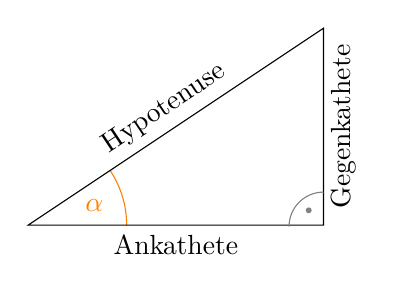
\begin{tikzpicture}[scale=1.25]
        \draw[orange] (1,0) arc[radius=1, start angle=0, end angle=33.7];
        \node[orange] at (16.85:0.7) {$\alpha$};
        \draw (0,0) -- 
            node[below] {Ankathete} (3,0) -- 
            (3,2) -- 
            node[rotate=33.7,above] {Hypotenuse} cycle;
            \draw[gray] (3,0.335) arc[radius=0.35, start angle=90, end angle=180];
            \fill[gray] (2.85,0.15) circle[radius=.3mm];
            \node[rotate=90] at (3.2,1) {Gegenkathete};
    \end{tikzpicture}

    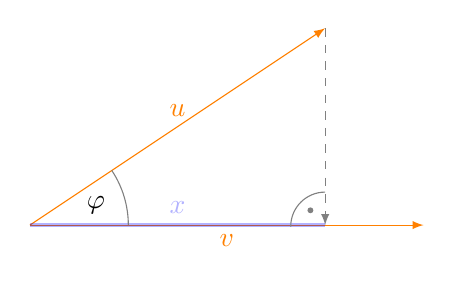
\begin{tikzpicture}[scale=1.25]
        \draw[-latex,orange] (0,0) -- node[above] {$u$} (3,2);
        \draw[-latex,orange] (0,0) -- node[below] {$v$} (4,0);
        \draw[-latex,dashed,gray] (3,2) -- (3,0);
        \draw[ultra thick, opacity=0.3,blue] (0,0) -- node[above] {$x$} (3,0);
        \draw[gray] (3,0.335) arc[radius=0.35, start angle=90, end angle=180];
        \fill[gray] (2.85,0.15) circle[radius=.3mm];
        \draw[gray] (1,0) arc[radius=1, start angle=0, end angle=33.7];
        \node at (16.85:0.7) {$\varphi$};
    \end{tikzpicture}
\end{multicols}
Unsere Vektoren bilden zunächst noch kein Dreieck -- und erst recht kein rechtwinkliges Dreieck. Um das zu ändern, 
verbinden wir so wie im rechten Bild dargestellt die Pfeilspitze des Vektors $u$ so mit dem Vektor $v$, 
dass die Verbindung (grau gestrichelt dargestellt) genau in einem rechten Winkel auf $v$ trifft. Die blau hinterlegte
Strecke $x$ ist dann die Ankathete in unserem rechtwinkligen Dreieck und $u$ ist die Hypotenuse in diesem Dreieck. Wenn
wir jetzt die Länge von $x$ (der Ankathete) durch die Länge von $u$ (die Hypotenuse) teilen, erhalten wir den Cosinus
von $\varphi$:
\[\cos(\varphi)=\frac{\abs{x}}{\abs{u}}.\]
\begin{example}[ex:angle-between-vectors-without-dot-product]{}
    \parpic[r]{
        \tikz{
        \begin{axis}[defgrid, domain=0:4, y=1cm, x=1cm, ymin=0, ymax=4, xmin=0, xmax=4, xtick={1,...,4}, ytick={1,...,4}]
            \node at (67.5:0.7) {$\varphi$};
            \draw[gray] ($(2,2) + (135:0.5)$) arc[radius=0.5, start angle=135, end angle=225];
            \fill[gray] ($(2,2) + (180:0.3)$) circle[radius=.4mm];
            \draw[gray] (45:1) arc[radius=1, start angle=45, end angle=90];
            \draw[-latex, ultra thick, orange] (0,0) -- node[right] {$u$} (0,4);
            \draw[-latex, ultra thick, orange] (0,0) -- (3,3) node[above] {$v$};
            \draw[-latex, ultra thick, blue!30] (0,0) -- node[above] {$x$} (2,2);
            \draw[-latex,dashed,gray, thick] (0,4) -- (2,2);
        \end{axis}
        }
    }
    \picskip{8}
    Rechts siehst du die Vektoren $u=\vectwo{0}{4}$ und \mbox{$v=\vectwo{3}{3}$}. Wir verbinden die Pfeilspitze von $u$
    so mit dem Vektor $v$, dass der eingezeichnete rechte Winkel entsteht. Die Ankathete des entstehenden rechtwinkligen
    Dreiecks ist blau eingezeichnet und gehört zum Vektor $x=\vectwo{2}{2}$. Die Hypotenuse ist $u$. Wenn wir die Längen
    von $x$ und $u$ ausrechnen, erhalten wir
    \[\abs{x}=\sqrt{2^2+2^2}=\sqrt{8}\text{ und }\abs{v}=\sqrt{0^2+4^2}=\sqrt{16}=4.\]
    Damit können wir den Cosinus von $\varphi$ berechnen:
    \[\cos(\varphi)=\frac{\sqrt{8}}{4}=\frac{\sqrt{4}\cdot\sqrt{2}}{4}=\frac{2\sqrt{2}}{4}=\frac{\sqrt{2}}{2}.\]
    Nun können wir, etwa mit dem Befehl \circlelbl{$\cos^{-1}$} eines Taschenrechners, den Winkel 
    $\varphi=\arccos\bigl(\frac{\sqrt{2}}{2}\bigr)=45^\circ$ bestimmen. Die beiden Vektoren schließen also einen Winkel
    von $45^\circ$ ein.
\end{example}
Wie du die Länge von $u$ ausrechnen kannst, hast du bereits im letzten Abschnitt gelernt: Der Vektor $u=\vectwo{u_1}{u_2}$
hat die Länge $\abs{u}=\sqrt{u_1^2+u_2^2}$. Schwieriger ist es, die Länge von $x$ auszurechnen. Um diese Länge zu berechnen,
müssen wir zunächst das \textbf{Skalarprodukt} der Vektoren kennenlernen (dies ist \emph{nicht} das gleiche wie Skalarmultiplikation!).
Das Skalarprodukt zweier Vektoren erhalten wir, wenn wir sie nebeneinander schreiben und dann immer die Einträge miteinander
multiplizieren, die nebeneinander stehen:
\begin{center}
    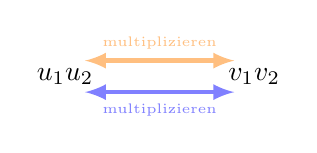
\begin{tikzpicture}
        \node at (-1.2,0) {$\vectwo{u_1}{u_2}$};
        \node at (1.2,0) {$\vectwo{v_1}{v_2}$};
        \draw[ultra thick, latex-latex, orange!50] (-0.95,0.2) -- node[above] {\tiny multiplizieren} (0.95,0.2);
        \draw[ultra thick, latex-latex, blue!50] (-0.95,-0.2) -- node[below] {\tiny multiplizieren} (0.95,-0.2);
    \end{tikzpicture}
\end{center}
Die Summe aller Ergebnisse, die wir bei den Multiplikationen erhalten, ist das Skalarprodukt unserer Vektoren:
\[\inprod{\vectwo{u_1}{u_2}}{\vectwo{v_1}{v_2}}=\textcolor{orange}{u_1v_1}+\textcolor{blue}{u_2v_2}\]
\begin{example}{}
    Wir berechnen das \emph{Skalarprodukt} der Vektoren $\vectwo{2}{3}$ und $\vectwo{4}{3}$. Wir multiplizieren also zuerst
    die nebeneinander stehenden Einträge:
    \begin{center}
        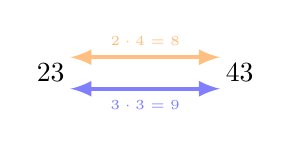
\begin{tikzpicture}
            \node at (-1.2,0) {$\vectwo{2}{3}$};
            \node at (1.2,0) {$\vectwo{4}{3}$};
            \draw[ultra thick, latex-latex, orange!50] (-0.95,0.2) -- node[above] {\tiny $2\cdot 4=8$} (0.95,0.2);
            \draw[ultra thick, latex-latex, blue!50] (-0.95,-0.2) -- node[below] {\tiny $3\cdot 3=9$} (0.95,-0.2);
        \end{tikzpicture}
    \end{center}
    Anschließend müssen wir die Ergebnisse noch addieren und erhalten das Skalarprodukt
    \[\inprod{\vectwo{2}{3}}{\vectwo{4}{3}}=\textcolor{orange}{8}+\textcolor{blue}{9}=17.\]
\end{example}
Das Skalarprodukt ist also wie folgt definiert:
\begin{definition}{Standardskalarprodukt}
    Für zwei Vektoren $a=\vectwo{a_1}{a_2}$
    und $b=\vectwo{b_1}{b_2}$
    ist das \textbf{Standardskalarprodukt} von $a$ und $b$, geschrieben als $\inprod{a}{b}$, definiert durch
    \[\inprod{a}{b}:=a_1b_1+a_2b_2.\]
\end{definition}
\parpic[r]{
    \tikz{
    \begin{axis}[defgrid, domain=0:4, y=1cm, x=1cm, ymin=0, ymax=4, xmin=0, xmax=4, xtick={1,...,4}, ytick={1,...,4}]
        \node at (67.5:0.7) {$\varphi$};
        \draw[gray] ($(2,2) + (135:0.5)$) arc[radius=0.5, start angle=135, end angle=225];
        \fill[gray] ($(2,2) + (180:0.3)$) circle[radius=.4mm];
        \draw[gray] (45:1) arc[radius=1, start angle=45, end angle=90];
        \draw[-latex, ultra thick, orange] (0,0) -- node[right] {$u$} (0,4);
        \draw[-latex, ultra thick, orange] (0,0) -- (3,3) node[above] {$v$};
        \draw[-latex, ultra thick, blue!30] (0,0) --  node[above] {$x$} (2,2);
        \draw[-latex,dashed,gray, thick] (0,4) -- (2,2);
        \node[blue!75,right] at (1.15,0.65) {$\abs{x}=\frac{\inprod{u}{v}}{\abs{v}}$};
        \draw[blue!75,decoration={brace,mirror,raise=5pt},decorate] (0,0) -- (2,2);
    \end{axis}
    }
}
\picskip{12}
Was hat das Skalarprodukt nun aber mit Winkeln zu tun? Wenn wir die Pfeilspitze eines Vektors $u$ wie bereits zu Beginn 
dieses Abschnitts beschrieben mit dem Vektor $v$ verbinden, gibt uns das Skalarprodukt der Vektoren $u$ und $v$ an, wie
lang die rechts blau eingezeichnete Ankathete $x$ des entstehenden rechtwinkligen Dreiecks ist, wenn man ihre Länge mit der
Länge von $v$ multipliziert. Es gilt also
\[\abs{x}\cdot \abs{v}=\inprod{u}{v}\]
(das ist überhaupt nicht offensichtlich und wir werden diesen Zusammenhang im weiterführenden 
Wissen beweisen). Wenn wir diese Gleichung durch $\abs{v}$ teilen, erhalten wir also die Länge von $\abs{x}$ als
\[\abs{x}=\frac{\inprod{u}{v}}{\abs{v}}.\]
Diesen Wert können wir jetzt nutzen, um den Cosinus des Winkels $\varphi$ vollständig zu berechnen:
\[\cos(\varphi)
=\frac{\textcolor{blue!75}{\abs{x}}}{\textcolor{orange}{\abs{u}}}
=\frac{\textcolor{blue!75}{\inprod{u}{v}}}{\textcolor{orange}{\abs{u}}\cdot\textcolor{blue!75}{\abs{v}}}\]
\begin{example}[ex:angle-between-vectors-with-dot-product]{}
    Wir haben in Beispiel \ref{ex:angle-between-vectors-without-dot-product} bereits den Winkel zwischen den Vektoren
    $u=\vectwo{0}{4}$ und $v=\vectwo{3}{3}$ berechnet. Die Länge der Ankathete haben wir dabei durch eine Zeichnung 
    herausgefunden. Mit dem Skalarprodukt können wir diese Länge auch direkt berechnen. Dafür berechnen wir zunächst das
    Skalarprodukt der Vektoren $u$ und $v$:
    \[\inprod{u}{v}=\inprod{\vectwo{0}{4}}{\vectwo{3}{3}}=0\cdot 3+4\cdot 3=12\]
    Der Vektor $v$ hat die Länge $\abs{v}=\sqrt{3^2+3^2}=\sqrt{18}$. In Beispiel \ref{ex:angle-between-vectors-without-dot-product}
    haben wir bereits ausgerechnet, dass $\abs{u}=4$ gilt. Der Cosinus von $\varphi$ ist also
    \[\cos(\varphi)=\frac{\inprod{u}{v}}{\abs{u}\cdot\abs{v}}=\frac{12}{4\cdot\sqrt{18}}.\]
    Das Ergebnis sieht zwar anders aus als in Beispiel \ref{ex:angle-between-vectors-without-dot-product}, aber wir
    können nachrechnen, dass es sich tatsächlich genau um die gleiche Zahl handelt:
    \[\frac{12}{4\sqrt{18}}=\frac{3}{\sqrt{9}\cdot\sqrt{2}}=\frac{3}{3\sqrt{2}}=\frac{1}{\sqrt{2}}=\frac{\sqrt{2}}{2}\]
\end{example}
\begin{advanced}{Das Skalarprodukt als orthogonale Projektion}
\end{advanced}

Zum Abschluss dieses Abschnitts schauen wir uns noch ein paar Spezialfälle an, die auftreten können, wenn wir den
Winkel zwischen zwei Vektoren berechnen.

\begin{example}{}
    \parpic[r]{
        \tikz{
        \begin{axis}[defgrid, domain=0:4, y=1cm, x=1cm, ymin=0, ymax=4, xmin=0, xmax=4, xtick={1,...,4}, ytick={1,...,4}]
            \node at (45:0.4) {$\varphi$};
            \draw[gray] (0:.75) arc[radius=0.75, start angle=0, end angle=90];
            \draw[-latex, ultra thick, orange!70] (0,0) -- node[right] {$u$} (0,4);
            \draw[-latex, ultra thick, orange!70] (0,0) -- node[above] {$v$} (3,0);
            \draw[-latex,dashed,black!80, thick] (0,4) -- (0,0);
        \end{axis}
        }
    }
    \picskip{8}
    Wir berechnen den Winkel $\varphi$ zwischen den Vektoren $u=\vectwo{0}{4}$ und $v=\vectwo{3}{0}$, die rechts abgebildet sind.
    Wie wir jetzt wissen, gilt
    \[\cos(\varphi)=\frac{\inprod{u}{v}}{\abs{u}\cdot\abs{v}}.\]
    Wenn wir das Skalarprodukt berechnen, ergibt sich $\inprod{\vectwo{0}{4}}{\vectwo{3}{0}}=0\cdot 3+4\cdot 0=0$.
    
    Mit einem Blick auf das Bild rechts siehst du auch, wieso: Die beiden Vektoren $u$ und $v$ stehen senkrecht zueinander,
    sie schließen also einen Winkel von $90^\circ$ ein. Die Pfeilspitze von $u$ liegt dadurch genau über dem Startpunkt
    von $v$. Die Verbindung zwischen der Pfeilspitze von $u$ und dem Vektor $v$, die in einem rechten Winkel auf $v$ trifft,
    trifft genau beim Startpunkt beider Vektoren auf $v$ (du siehst den grauen Pfeil, wenn du genau hinsiehst, auch im Bild). 
    
    Die Strecke, die wir sonst blau eingezeichnet haben,
    hat hier deshalb die Länge 0. Das Skalarprodukt zweier Vektoren wird also genau dann 0, wenn die beiden Vektoren
    senkrecht zueinander stehen.
\end{example}
Wenn wir die Spitze eines Vektors $u$ so mit $v$ verbinden wollen, dass die Verbindungslinie senkrecht auf $v$ trifft,
aber $u$ bereits selbst senkrecht zu $v$ ist (wie im letzten Beispiel), dann landet die Verbindungslinie genau im Startpunkt von $u$ und $v$. Die
Ankathete, die wir vorher immer als blaue Linie gesehen haben, verschwindet dann und hat die Länge 0. Zwei Vektoren $u$
und $v$, die einen rechten Winkel einschließen, haben damit stets das Skalarprodukt 0.

Alternativ kannst du auch ausrechnen, dass $\cos(90^\circ)=0$ gilt. Für zwei Vektoren, die einen rechten Winkel einschließen,
ist also
\[\frac{\inprod{u}{v}}{\abs{u}\cdot\abs{v}}=\cos(\varphi)=\cos(90^\circ)=0.\]
Das ist nur möglich, wenn der Zähler des Bruchs auf der linken Seite 0 ist, also müssen zwei senkrecht zu einander stehende
Vektoren das Skalarprodukt 0 haben. Wir halten diese Beobachtung in der folgenden Definition fest:
\begin{definition}{Senkrechte Vektoren}
    Zwei Vektoren $u$ und $v$ heißen \textbf{senkrecht} (oder \textbf{orthogonal}) zu einander, falls ihr Skalarprodukt
    null ist, d.h. $\inprod{u}{v}=0$.
\end{definition}
Schließlich kann es noch passieren, dass zwei Vektoren genau in die gleiche Richtung zeigen und damit einen Winkel von
$0^\circ$ einschließen.
\begin{example}{}
    \parpic[r]{
        \tikz{
        \begin{axis}[defgrid, domain=0:4, y=1cm, x=1cm, ymin=0, ymax=3, xmin=0, xmax=4, xtick={1,...,4}, ytick={1,...,3}]
            \draw[-latex, ultra thick, orange!70] (0,0) -- (4,2);
            \draw[-latex, ultra thick, orange] (0,0) -- node[above] {$u$} (2,1);
            \node[orange!70] at (3.2,1.8) {$v$};
        \end{axis}
        }
    }
    \picskip{7}
    Die Vektoren $u=\vectwo{2}{1}$ und $v=\vectwo{4}{2}$ zeigen in die gleiche Richtung. Sie schließen einen
    Winkel von $0^\circ$ ein. Vermutlich hast du bereits bemerkt, dass $v$ einfach nur doppelt so lang wie $u$ ist und
    dass
    \[2\cdot\vectwo{2}{1}=\vectwo{4}{2}\]
    gilt. Vektoren können nur dann in die gleiche Richtung zeigen, wenn sie ein Vielfaches von einander sind, also wenn
    du einen der Vektoren (in diesem Fall $u$) so mit einer Zahl multiplizieren kannst, dass du den anderen Vektor 
    erhältst (in diesem Fall $v$).
\end{example}
Du hast bereits im letzten Abschnitt gelernt, dass sich die Richtung eines Vektors nicht ändert, wenn du ihn mit einer
Zahl (einem Skalar) multiplizierst: Die Vektoren
\[\vectwo{v_1}{v_2}\text{ und }\lambda\cdot \vectwo{v_1}{v_2}=\vectwo{\lambda v_1}{\lambda v_2}\]
zeigen immer in die gleiche Richtung. Zwei Vektoren, die in die gleiche Richtung zeigen, nennt man \textbf{linear abhängig}.
\begin{definition}{Lineare Abhängigkeit}
    Zwei Vektoren $u=\vectwo{u_1}{u_2}$ und $v=\vectwo{v_1}{v_2}$ heißen \textbf{linear abhängig}, falls eine Zahl 
    $\lambda\in\R$ existiert mit
    \[\lambda\cdot\vectwo{u_1}{u_2}=\vectwo{v_1}{v_2}.\]
    Ansonsten heißen die Vektoren $u$ und $v$ \textbf{linear unabhängig}.
\end{definition}
\begin{example}{Parallel = linear abhängig}

\end{example}

\begin{nutshell}{Das Skalarprodukt}
    
\end{nutshell}
    Todo: $\arccos$ in erstem Beispiel erläutern, parallel = linear abhängig und diese Zusammenfassung
\end{document}